\chapter{Data}
\label{cha:data}

This chapter describes the spatiotemporal dataset used in the thesis project.
The data provider is briefly mentioned, followed by the structure of the data.
This chapter also mentions issues encountered in the data set.

\section{Background}
The dataset was provided by Östgötatrafiken AB and contains \todo{300?}GB of data.
Östgötatrafiken AB is owned by Östergötland County and is responsible for the public transportation in the county.
This thesis project only analysed the bus data available in the given data set.
The dataset is a collection of documents, where one document represents a full day of data.
A typical day has a document size of around \todo{2.5?}GB.

\subsection{Data Gathering}
The process of gathering the data used in this thesis project can be generally described by the following simplified procedure:
\begin{enumerate}
    \item Each Östgötatrafiken AB bus is running a system collecting data from sensors installed inside the bus.
    \item The system collects the sensor data and transmits it to a central server or database.
    \item A log containing all events for a full day is created and stored as a document in a collection.
    \item The central server processes and analyses the data. The results from the data analysis is stored in the log.
\end{enumerate}

\begin{figure}
    \centering
    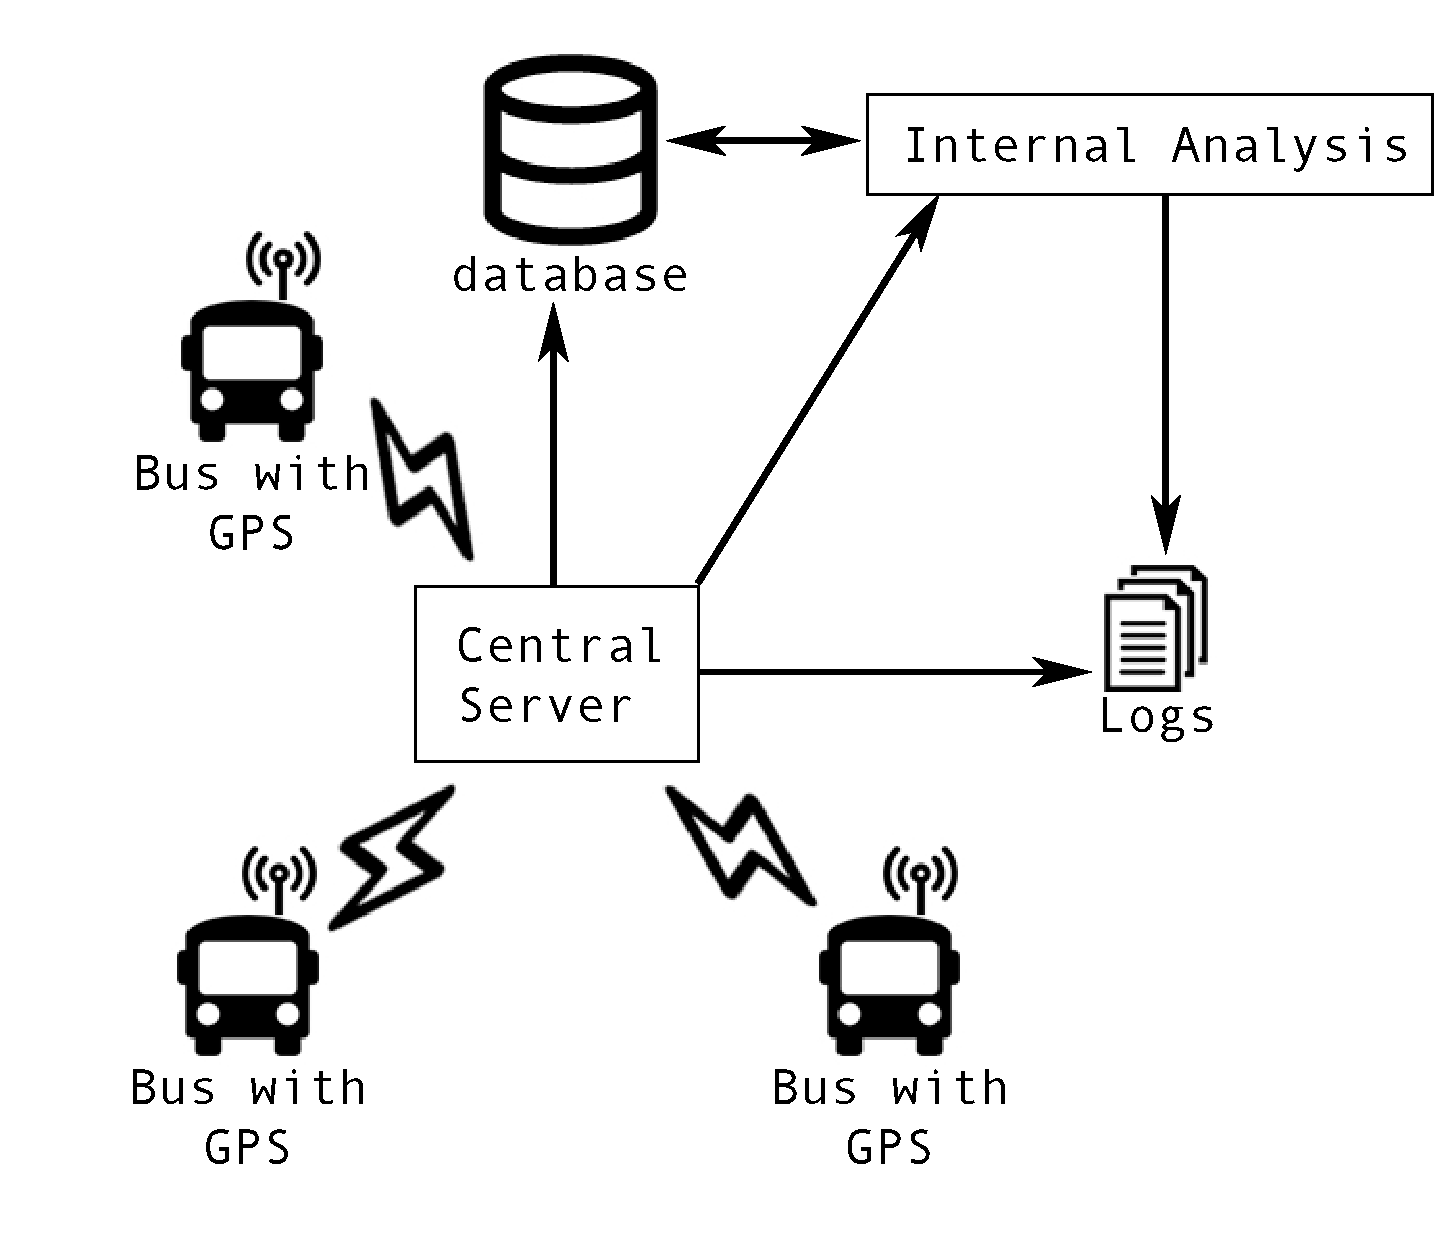
\includegraphics[width=0.75\textwidth]{figures/data-gathering}
    \caption{Simplified graph illustrating the data gathering process. Each bus is equipped with a GPS sensor and transmits its position to a central server/database.
    The dataset used in this thesis project is the log, which is a collection of documents.
    Each document contains the GPS data sent from all buses during a single day, together with data from the "Internal Analysis" component of the server.}
    \label{fig:data-gathering}
\end{figure}

Figure \ref{fig:data-gathering} illustrates the procedure.
The collection of logs is the dataset used in this thesis project.
The logs contain the GPS data from the buses and also events created by the "Internal Analysis" component in the system.
The "Internal Analysis" component is simplified and is beyond the scope of this thesis project.

\section{Structure}
A document in the dataset is made up of a large number of events representing a single day.
A single day typically contains roughly 21 \todo{Is it interesting to plot this exact number and its variance?} million events.  
Each event is represented by a single line of text.
An event can be split into two groups: a header and a body.
There are different types of events reported during the span of a single day.
Each type has its own header and body structure.

\subsection{Event Example}

\begin{figure}[ht!]
    \centering
    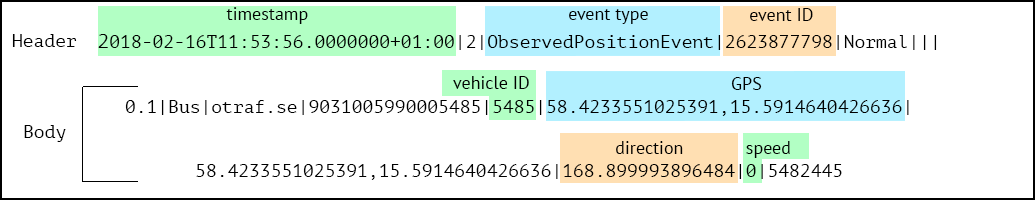
\includegraphics[width=\textwidth]{figures/data-example-1}
    \caption{Example of a raw \texttt{ObservedPositionEvent} entry.
    The header and the body is separated by \texttt{|||}.
    Each parameter in the header and body is separated by a single \texttt{|}.
    Key parameters for the \texttt{ObservedPositionEvent} event type is highlighted.}
    \label{fig:data-ex-1}
\end{figure}

Figure \ref{fig:data-ex-1} illustrates an event with the event type \texttt{ObservedPositionEvent}.
The header is defined as all the parameters before the \texttt{|||} separator.
All the parameters after the separator is defined as the body of the event.
In this example the header and body contain seven key parameters: 
\begin{itemize}
    \item \textit{Timestamp:} A timestamp (\texttt{2018-02-16T11:53:56.0000000+01:00}), which is the timestamp from the system running on the bus.
    \item \textit{Event Type:} The event type (\texttt{ObservedPositionEvent}).
    \item \textit{Event ID:} The event id (\texttt{2623877798}). This is a number set by the system responsible for collecting the data from all buses.
    It is incremented for every event added to the log by either the database system or the "Internal Analysis" component in Figure \ref{fig:data-gathering}.
    \item \textit{Vehicle ID:} Unique ID for the bus transmitting its position.
    \item \textit{GPS:} The GPS position of the bus in latitude and longitude.
    \item \textit{Direction:} The direction of the bus.
    \item \textit{Speed:} The current speed of the bus.
\end{itemize}

\subsection{Event Types}
The dataset contains 20 unique event types.
Figure \ref{fig:types-barplot} visualises the distribution of event types for a random day \todo{Should we do a boxplot instead of the whole dataset? Will take a lot of time to create!} in the dataset.
The figure only gives an indication of what the true distribution could be, as it is computationally expensive to calculate the true distribution for the given dataset, due to its size.
Knowledge about the true distribution is not required in order to reason about the event types.
As the figure shows, the majority of events that occur are of the type \texttt{ObservedPositionEvent}, which is the event containing an updated GPS position for a vehicle.

\begin{figure}[ht!]
    \centering
    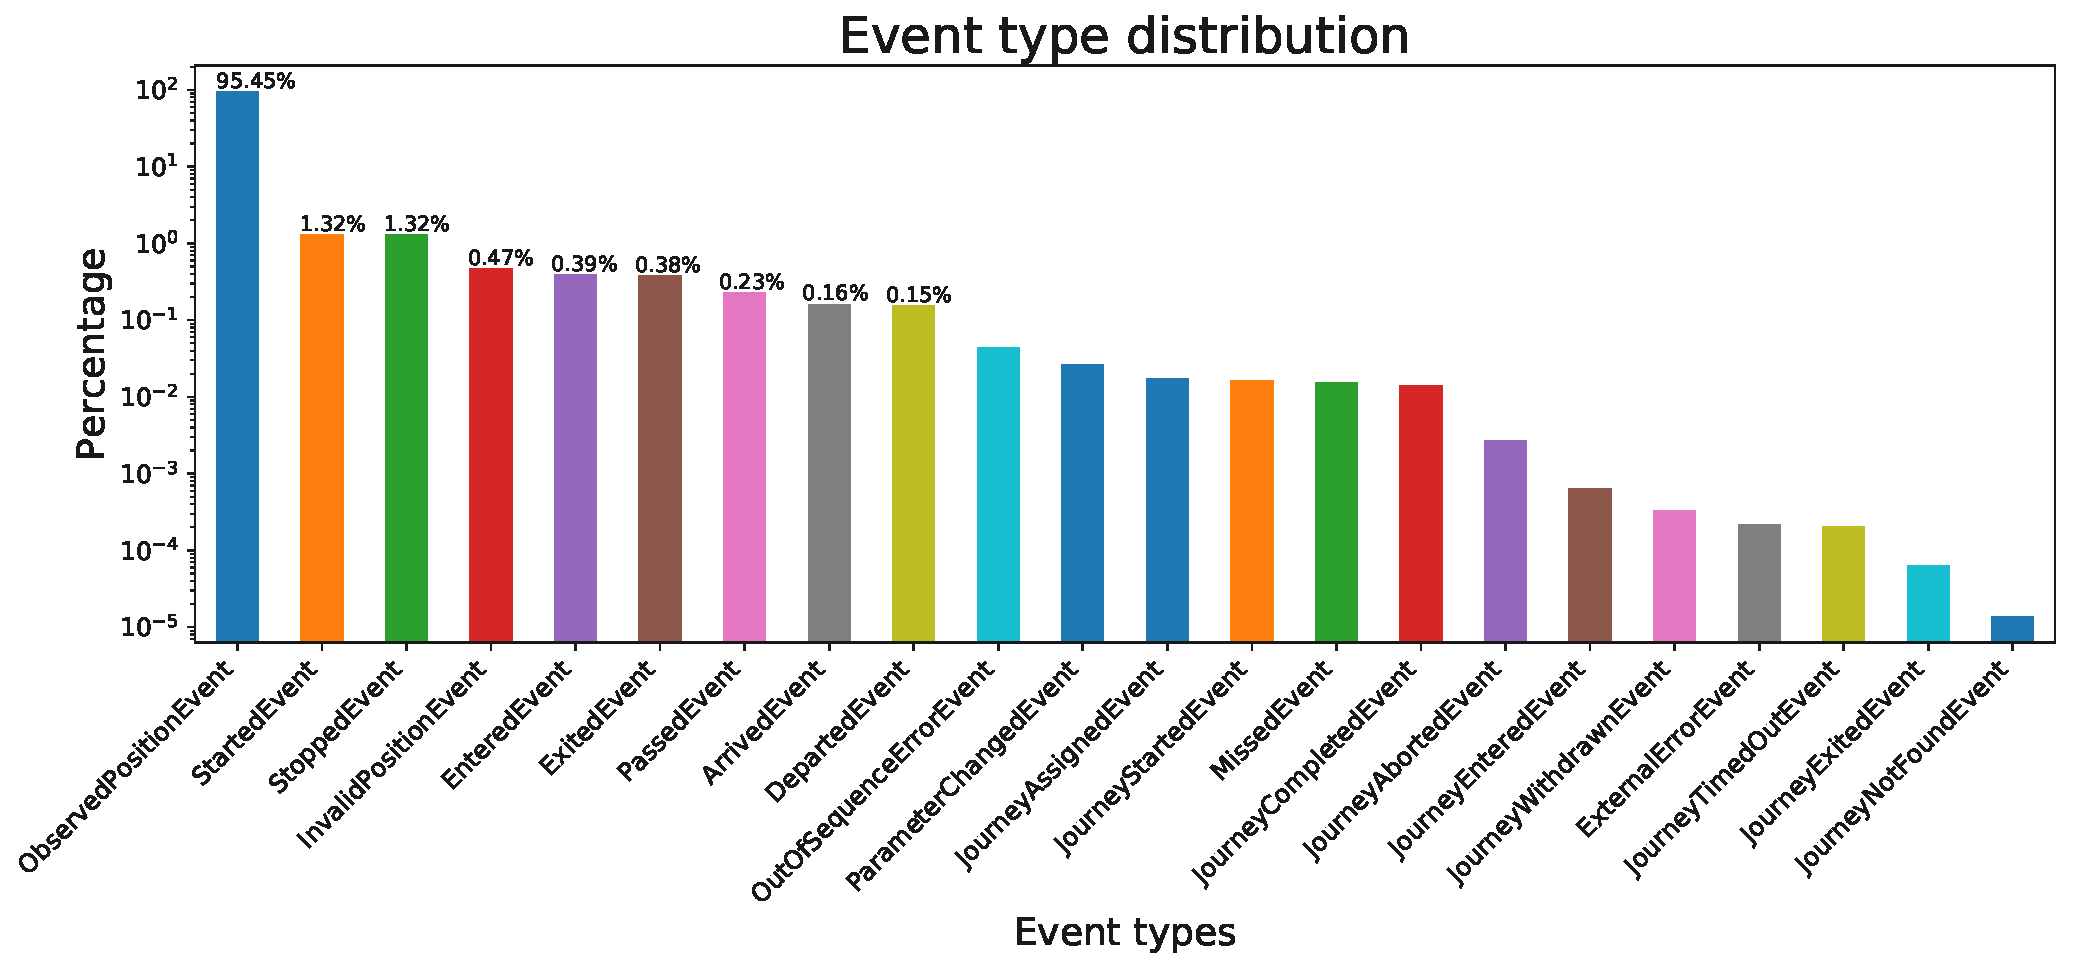
\includegraphics[width=\textwidth]{figures/types_barplot}
    \caption{The distribution of event types for a random day in the dataset.}
    \label{fig:types-barplot}
\end{figure}

Of the 20 event types available in the dataset, this thesis project only used 11 of them.
The events to use were chosen by analysing the log for a single day in great detail.
Event types which occurred rarely and seemingly random were discarded, as no pattern could be determined for them.
The \texttt{InvalidPositionEvent} type only contains the GPS position of the vehicle.
The valid \texttt{ObservedPositionEvent} type also contains the \textit{Speed} and \textit{Direction} parameters.
The GPS position of the \texttt{InvalidPositionEvent} events were always the same coordinates.
In this thesis project the \texttt{InvalidPositionEvent} type was discarded, due to the missing parameters and static GPS position.

The 11 event types used in this thesis project were:
\begin{itemize}
    \item \textit{ObservedPositionEvent:}
    \item \textit{StartedEvent:}
    \item \textit{StoppedEvent:}
    \item \textit{InvalidPositionEvent:}
    \item \textit{ExitedEvent:}
    \item \textit{EnteredEvent:}
    \item \textit{PassedEvent:}
    \item \textit{DepartedEvent:}
    \item \textit{ArrivedEvent:}
    \item \textit{ParameterChangedEvent:}
    \item \textit{JourneyStartedEvent:}
    \item \textit{JourneyAssignedEvent:}
\end{itemize}


